\subsection*{Problema 09}

\textbf{Enunciado:} Evaluar la integral definida 
mediante la definición de sumas de Riemann:
\begin{align*}
\int_{1}^{2} (4 - x^2) \, dx
\end{align*}

\textbf{Solución:} 
Aplicamos la definición de la integral definida 
usando el límite de una suma de Riemann por la 
derecha. Dividimos el intervalo $[1, 2]$ en $n$ 
subintervalos de ancho igual a:
\begin{align*}
\Delta x = \dfrac{2 - 1}{n} = \dfrac{1}{n}
\end{align*}

Los puntos de muestreo son $x_i = 1 + \dfrac{i}{n}$. 
Evaluamos la función en estos puntos:
\begin{align*}
f(x_i) &= 4 - \left(1 + \dfrac{i}{n}\right)^2 \\
&= 4 - \left(1 + \dfrac{2i}{n} + \dfrac{i^2}{n^2}\right) \\
&= 3 - \dfrac{2i}{n} - \dfrac{i^2}{n^2}
\end{align*}

Planteamos la suma de Riemann:
\begin{align*}
S_n &= \sum_{i=1}^{n} f(x_i) \Delta x \\
&= \sum_{i=1}^{n} \left(3 - \dfrac{2i}{n} - \dfrac{i^2}{n^2}\right) \dfrac{1}{n}
\end{align*}

Distribuimos el término $\dfrac{1}{n}$ y 
separamos la sumatoria:
\begin{align*}
S_n &= \dfrac{3}{n}\sum_{i=1}^{n} 1 
- \dfrac{2}{n^2}\sum_{i=1}^{n} i 
- \dfrac{1}{n^3}\sum_{i=1}^{n} i^2
\end{align*}

Utilizamos las fórmulas conocidas para las 
sumas notables:
\begin{align*}
\sum_{i=1}^{n} 1 &= n \\
\sum_{i=1}^{n} i &= \dfrac{n(n+1)}{2} \\
\sum_{i=1}^{n} i^2 &= \dfrac{n(n+1)(2n+1)}{6}
\end{align*}

Sustituimos estas fórmulas en la expresión 
de $S_n$:
\begin{align*}
S_n &= \dfrac{3}{n}(n) 
- \dfrac{2}{n^2}\left[\dfrac{n(n+1)}{2}\right] \\
&\quad - \dfrac{1}{n^3}\left[\dfrac{n(n+1)(2n+1)}{6}\right]
\end{align*}

Simplificamos cada término algebraicamente:
\begin{align*}
S_n &= 3 - \dfrac{n+1}{n} 
- \dfrac{(n+1)(2n+1)}{6n^2} \\
&= 3 - \left(1 + \dfrac{1}{n}\right) 
- \dfrac{2n^2 + 3n + 1}{6n^2} \\
&= 2 - \dfrac{1}{n} - \left(\dfrac{1}{3} + \dfrac{1}{2n} + \dfrac{1}{6n^2}\right)
\end{align*}

Agrupamos los términos constantes y los que 
dependen de $n$:
\begin{align*}
S_n &= \left(2 - \dfrac{1}{3}\right) 
- \left(1 + \dfrac{1}{2}\right)\dfrac{1}{n} 
- \dfrac{1}{6n^2} \\
&= \dfrac{5}{3} - \dfrac{3}{2n} - \dfrac{1}{6n^2}
\end{align*}

Finalmente, calculamos el límite cuando 
$n \to \infty$ para obtener el valor de la 
integral:
\begin{align*}
\int_{1}^{2} (4 - x^2) \, dx &= \lim_{n \to \infty} S_n \\
&= \lim_{n \to \infty} \left(\dfrac{5}{3} - \dfrac{3}{2n} - \dfrac{1}{6n^2}\right) \\
&= \dfrac{5}{3}
\end{align*}

El valor exacto de la integral definida es 
$\dfrac{5}{3}$ (aproximadamente $1.6667$).

\begin{figure}[H]
	\centering
	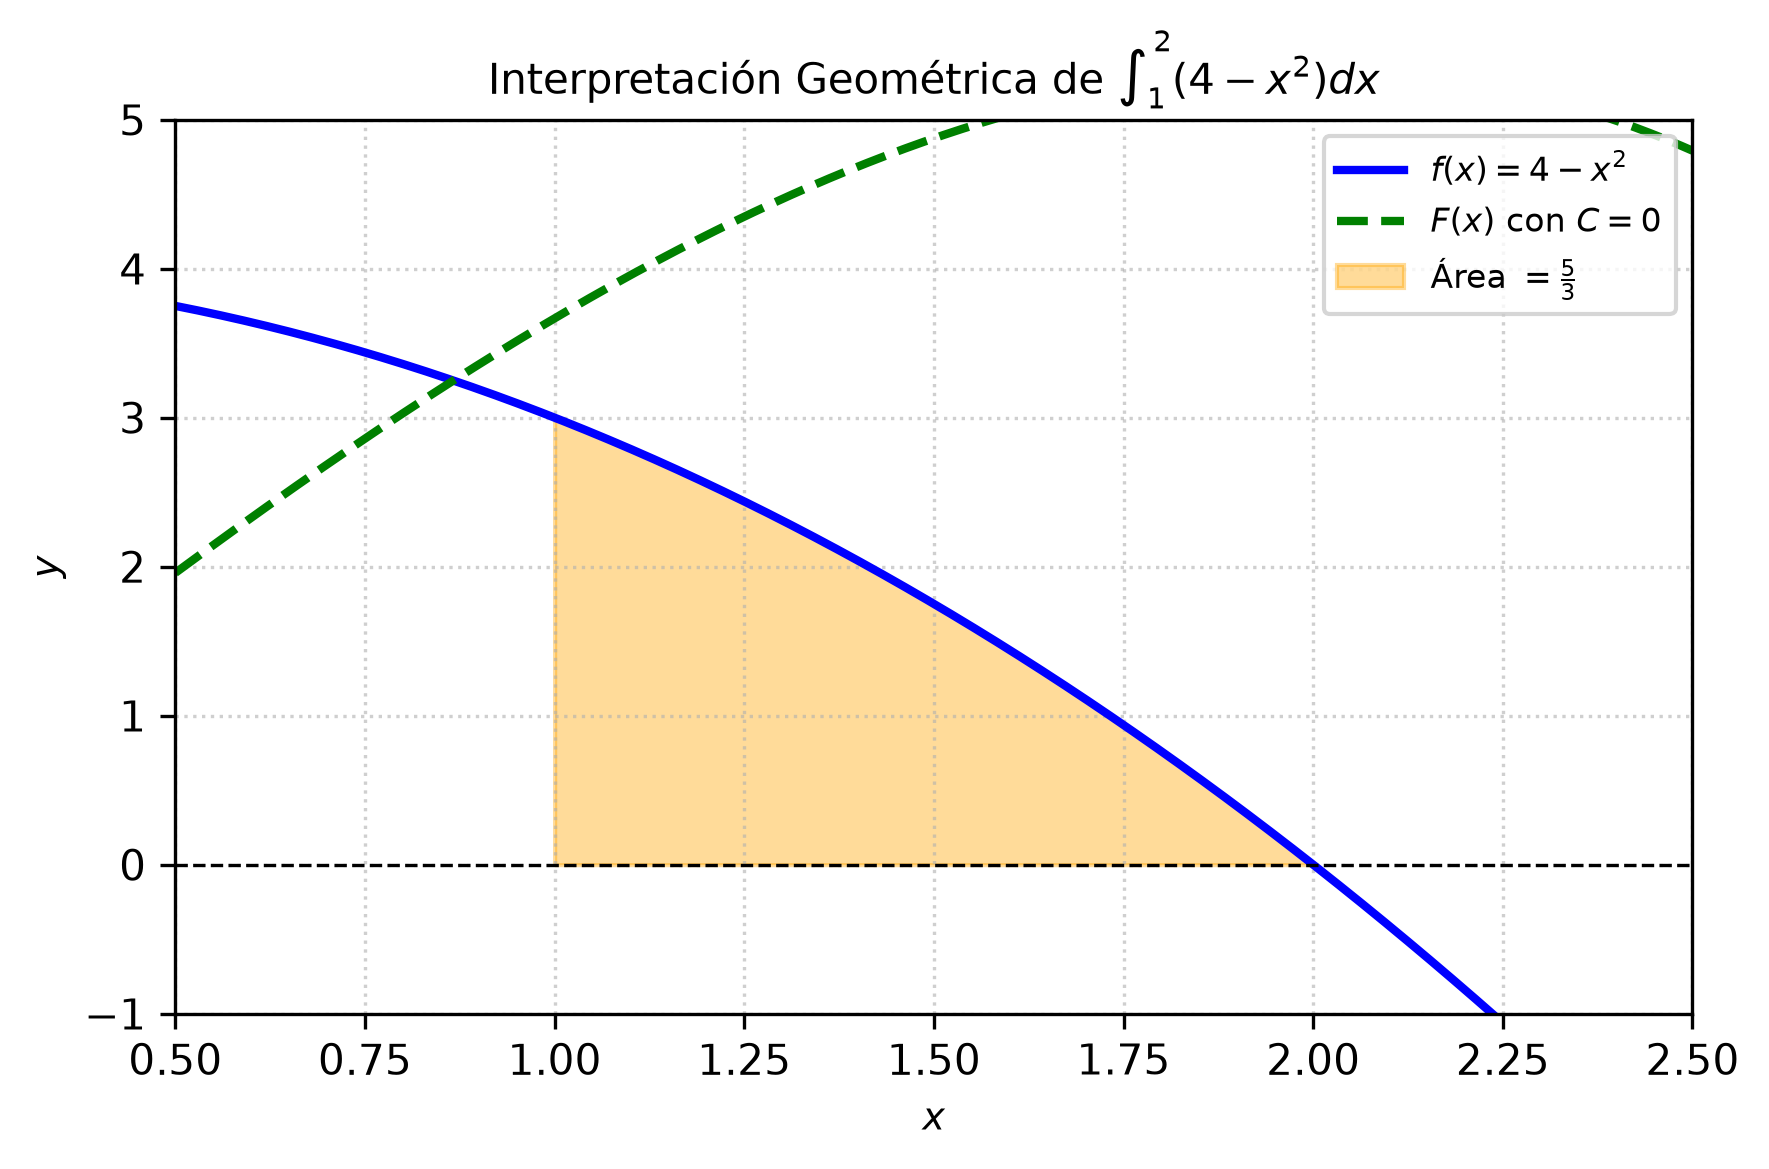
\includegraphics[width=\columnwidth]{semana_06/graficas/SEM06_P09_grafica.png}
	\caption{Representación gráfica de $f(x)$ y su antiderivada $F(x)$ evaluada para la constante de integración $C = 0$ (Problema 09).}
	\label{fig:problema09}
\end{figure}
